\subsection{Framework}
\begin{frame}{Framework}{Symfony2}



\begin{columns}[t]
  \begin{column}[l]{0.5\textwidth}
		\begin{block}{Histoire}
			\begin{itemize}
				\item Créé en 1998
				\item SensioLabs
				\item Framework aujourd'hui mature
			\end{itemize}
		\end{block}
	\end{column}
    \begin{column}[l]{0.5\textwidth}
		\begin{block}{Caractéristiques}
			\begin{itemize}
				\item MVC (Mojavi)
				\item ORM (Doctrine2)
				\item Template (Twig)
			\end{itemize}
		\end{block}
	\end{column}
\end{columns}
\end{frame}

\begin{frame}{Framework}{Structure des applications}
\begin{columns}[t]
    \begin{column}[l]{0.5\textwidth}
		\begin{block}{Bundle}
			\begin{itemize}
				\item module ou plugin
				\item portable
				\item facilement installable
				\item architecture MVC
			\end{itemize}
		\end{block}
	\end{column}
    \begin{column}[l]{0.5\textwidth}
		\begin{block}{Entity}
			\begin{itemize}
				\item classe
				\item paramétrable avec l'ORM
				\item contrôleur
				\item formulaires
			\end{itemize}
		\end{block}
	\end{column}
\end{columns}
\end{frame}

\begin{frame}{Framework}{ORM Doctrine2}
\begin{block}{Doctrine2}
\begin{itemize}
\item ORM populaire
\item GNU LGPL
\end{itemize}
\end{block}

\begin{block}{Intégration}
\begin{itemize}
\item ORM par défaut de Symfony
\item tag \texttt{@ORM}
\end{itemize}
\end{block}
\end{frame}

\subsection{Structure de l'application}
\begin{frame}{Structure}{Entité \emph{Terme}}
\lstinputlisting[language=PHP,morekeywords={class, public, function, return, private, namespace, use,as}]{./sources/Terme1.php}
\end{frame}

\begin{frame}{Structure}{Entité \emph{Terme}}
\lstinputlisting[language=PHP,morekeywords={class, public, function, return, private, namespace, use,as}]{./sources/Terme2.php}
\end{frame}

\begin{frame}{Structure}{Entité \emph{Concept}}
\lstinputlisting[language=PHP,morekeywords={class, public, function, return, private, namespace, use,as}]{./sources/Concept1.php}
\end{frame}

\begin{frame}{Structure}{Entité \emph{Concept}}
\lstinputlisting[language=PHP,morekeywords={class, public, function, return, private, namespace, use,as}]{./sources/Concept2.php}
\end{frame}

\begin{frame}{Structure}{Entité \emph{Concept}}
\lstinputlisting[language=PHP,morekeywords={class, public, function, return, private, namespace, use,as}]{./sources/Concept3.php}
\end{frame}

\begin{frame}{Structure}{Entité \emph{Concept}}
\lstinputlisting[language=PHP,morekeywords={class, public, function, return, private, namespace, use,as}]{./sources/Concept4.php}
\end{frame}

\begin{frame}{Structure}{Entité \emph{Concept}}
\lstinputlisting[language=PHP,morekeywords={class, public, function, return, private, namespace, use,as}]{./sources/Concept5.php}
\end{frame}

\begin{frame}{Structure}{Entité \emph{Concept}}
\lstinputlisting[language=PHP,morekeywords={class, public, function, return, private, namespace, use,as}]{./sources/Concept6.php}
\end{frame}

\subsection{Schéma relationnel généré}
\begin{frame}{Schéma relationnel généré}
\begin{description}
\item[terme](\underline{id})
\item[concept](\underline{id}, terme\_vedette\_id$^\#$, concept\_general\_id$^\#$)
\item[concept\_terme](\underline{concept\_id$^\#$, terme\_id$^\#$})
\item[concept\_concept](\underline{concept1\_id$^\#$, concept2\_id$^\#$})
\end{description}
\end{frame}

\subsection{Templates finaux}
\begin{frame}{Templates finaux}{Accueil}
\begin{center}
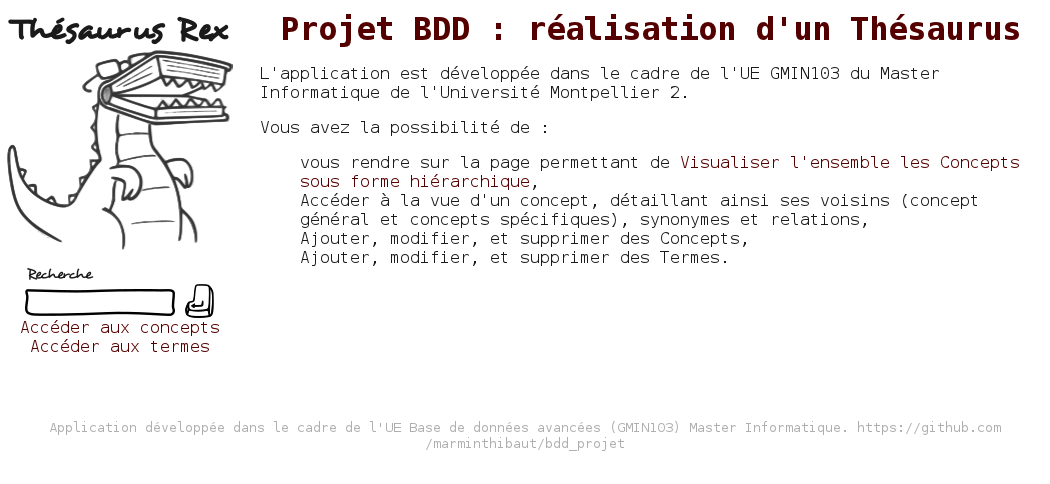
\includegraphics[width=\textwidth]{files/screen_accueil}
\end{center}
\end{frame}

\begin{frame}{Templates finaux}{Liste des concepts}
\begin{center}
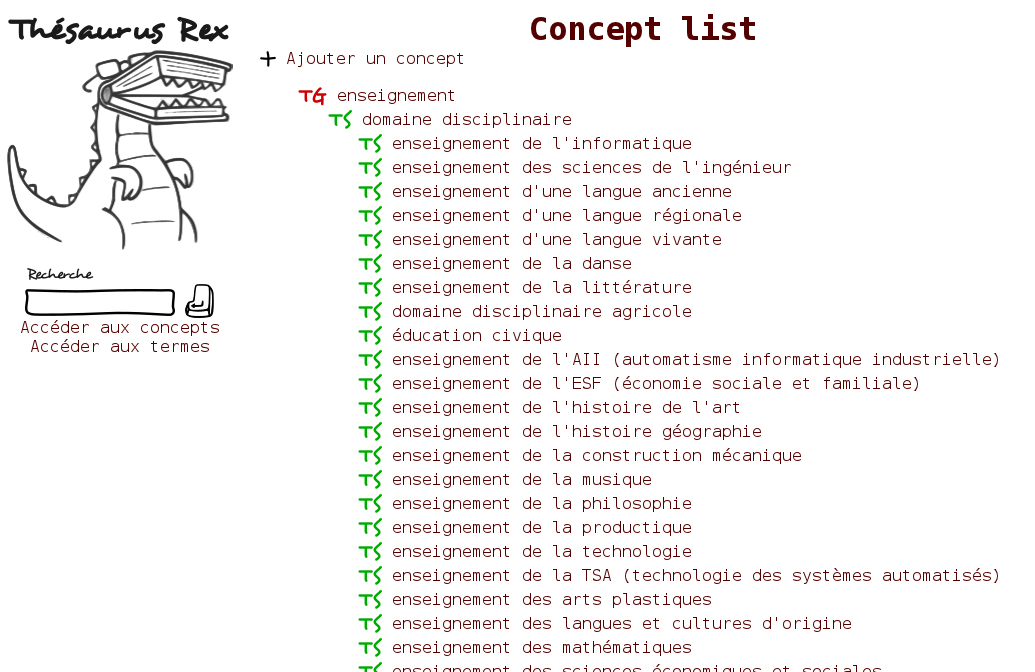
\includegraphics[width=\textwidth]{files/screen_concepts}
\end{center}
\end{frame}

\begin{frame}{Templates finaux}{Environnement sémantique direct}
\begin{center}
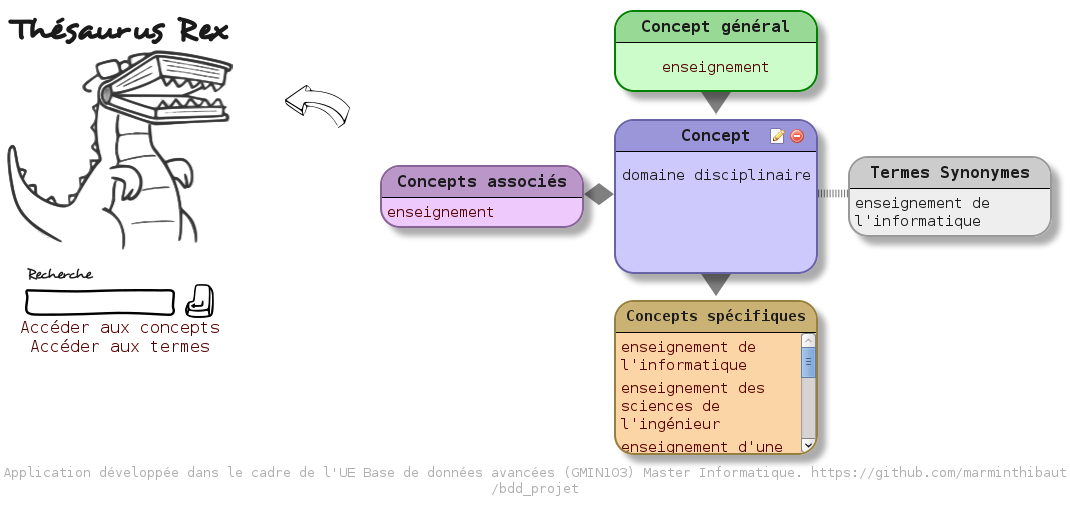
\includegraphics[width=\textwidth]{files/screen_concept}
\end{center}
\end{frame}

\begin{frame}{Templates finaux}{Ajout / Modification d'un concept}
\begin{center}
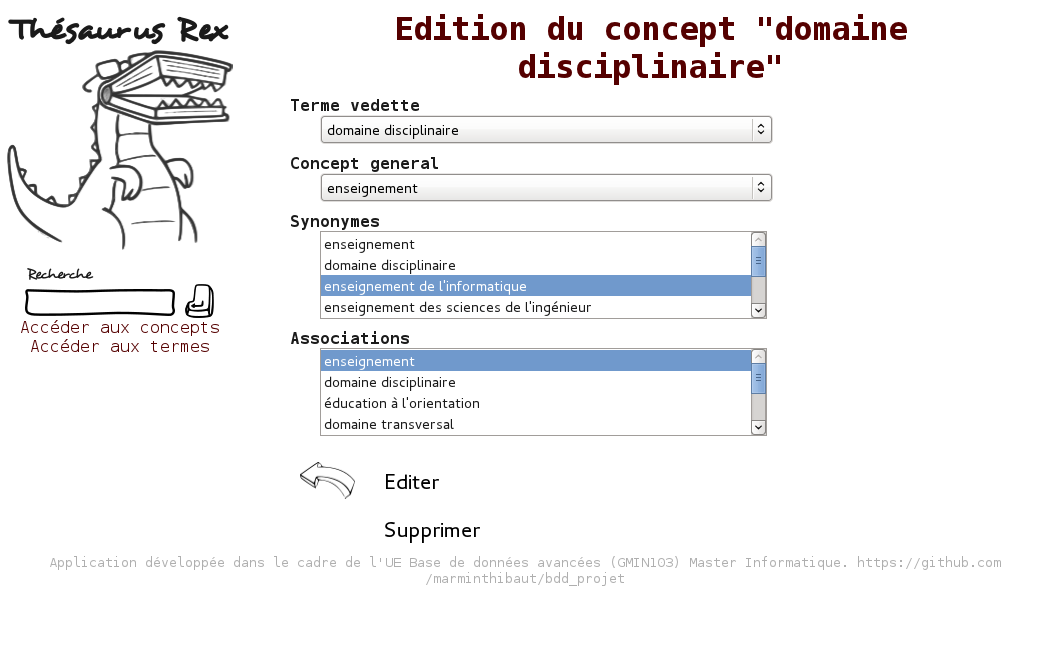
\includegraphics[width=\textwidth]{files/screen_concept_edit}
\end{center}
\end{frame}

\begin{frame}{Templates finaux}{Liste des termes}
\begin{center}
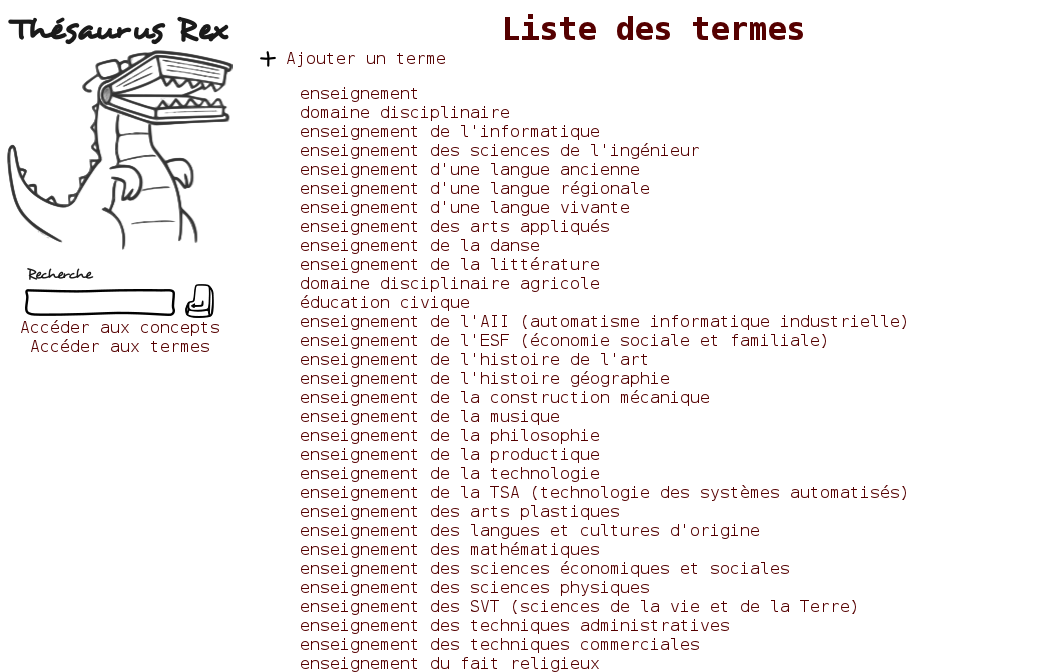
\includegraphics[width=\textwidth]{files/screen_termes}
\end{center}
\end{frame}

\begin{frame}{Templates finaux}{Modification d'un terme}
\begin{center}
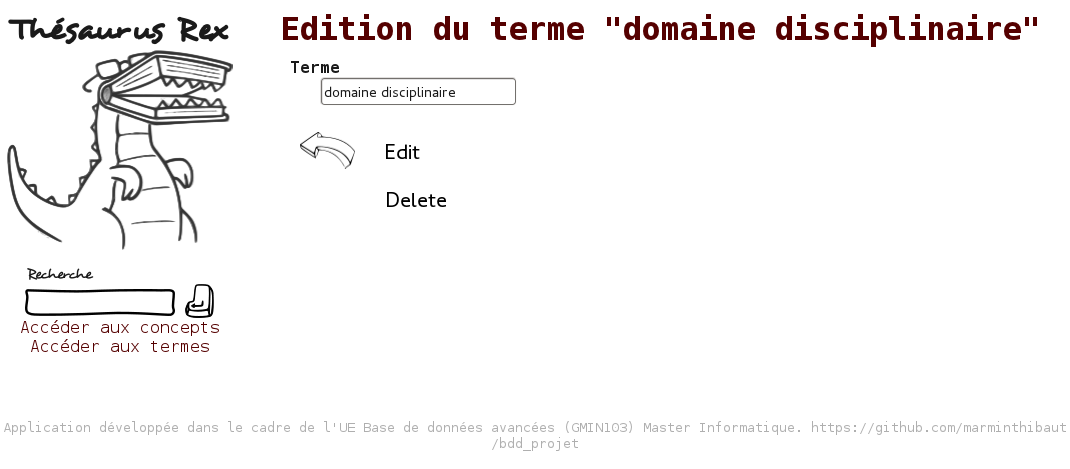
\includegraphics[width=\textwidth]{files/screen_terme_edit}
\end{center}
\end{frame}